% Template for ISBI paper; to be used with:
%          spconf.sty  - ICASSP/ICIP LaTeX style file, and
%          IEEEbib.bst - IEEE bibliography style file.
% --------------------------------------------------------------------------
\documentclass{article}
\usepackage{spconf,amsmath,graphicx}
\usepackage{cite}


% Example definitions.
% --------------------
\def\x{{\mathbf x}}
\def\L{{\cal L}}

% Title.
% ------
\title{A framework for One-Shot Lung Segmentation based on Learned Transformations
  }

  %  Data Argumentation via learned transformations for One-Shot Lung Segmentation
%
% Single address.
% ---------------
% \name{Author(s) Name(s)\thanks{Thanks to XYZ agency for funding.}}
% \address{Author Affiliation(s)}
%
% For example:
% ------------
%\address{School\\
%	Department\\
%	Address}
%
% Two addresses (uncomment and modify for two-address case).
% ----------------------------------------------------------
% \twoauthors
%  {Qiuli~Wang,Zhihuan~Li, Xiaohong~Zhang\sthanks{This work was partially supported by the National Natural Science Foundation of China (Grant No. 61772093), the Chongqing Major Theme Projects (Grant No. cstc2018jszx-cyztzxX0017). Qiuli~Wang and Zhihuan~Li contribute equally to this paper.}}
% 	{School of Big Data \& Software Engineering \\Chongqing University \\ Chongqing, 400000, China }
%  {Chen~Liu}
% 	{Radiology Department \\ The First Affiliated Hospital of \\Army Medical University \\ 400032, Chongqing, China}
%
% More than two addresses
% -----------------------
\name{Qiuli~Wang, Zhihuan~Li, Wei~Chen, Xiaohong~Zhang\sthanks{This work was partially supported by the National Natural Science Foundation of China (Grant No. 61772093), the Chongqing Major Theme Projects (Grant No. cstc2018jszx-cyztzxX0017). Qiuli~Wang and Zhihuan~Li contribute equally to this paper.}, Chen~Liu$^{\dagger}$, Lu~Yang$^{\ddagger}$}

\address{$^{\star}$School of Big Data \& Software Engineering, Chongqing University, Chongqing, 400044, China \\
$^{\dagger}$The First Affiliated Hospital of Army Medical University, 400032, Chongqing, China \\
    $^{\ddagger}$Chongqing University Cancer Hospital, Chongqing, 400044, China}
%
\begin{document}
%\ninept
%
\maketitle
%
\begin{abstract}
    Lung segmentation on CT (Computed Tomography) is a core step for many pieces of research on pulmonary diseases. Supervised methods have attained state-of-the-art accuracy; however, these methods heavily rely on supervised training with large labeled datasets. Labeling CT scans is a time-consuming task and different datasets acquired from different types of equipment may have various data characteristics.
    In this study, we present a framework for one-shot lung segmentation based on learned spatial and density transformations.
    Our framework requires only one segmented CT scan (source scan), and transform this scan using spatial and density transformations according to target scans. These target scans can be scans from another dataset or acquired from other types of equipment.
    Spatial and density transformations learns lung spatial deformation field and structural density using CNNs (Convolutional Neural Networks). Then we will train a supervised U-Net to segment lungs from CT scans using generated scans.
    As far as we know, we are the first to segment lungs using one-shot method.
    Our experiments demonstrate that our framework can achieve convincing results even if the source scan with label comes from another dataset.

\end{abstract}
%
\begin{keywords}
One-Shot, Lungs, Segmentation, CT (Computed Tomography), U-Net
\end{keywords}
%
\section{Introduction}
\label{sec:intro}

Lung segmentation on CT (Computed Tomography) is a core task for many studies on pulmonary diseases. Supervised learning methods attain state-of-the-art accuracy, but these models have some common drawbacks.

First of all, these supervised methods heavily rely on labeled datasets. Labeling lungs on CT scans requires significant expertise and time, since one case of chest CT contains about 200 slices. As a result, public available lung CT datasets are usually small. For example, VESSEL12 \cite{rudyanto2014comparing} contains 20 cases in training set, Lung CT Segmentation Challenge 2017 \cite{yang2017data} contains 60 cases. These datasets can not reflect the clinical diversity of lung structures.
Second, CT scans collected from different types of equipment vary in basic settings, which can cause different noise or image quality. Since supervised models' parameters are optimized according to these settings, the performances of the supervised models trained on the partial dataset are not stable on another dataset.

The drawbacks mentioned above have become limitations of clinical application for the supervised lung segmentation model.


\begin{figure*}[t]
    \centerline{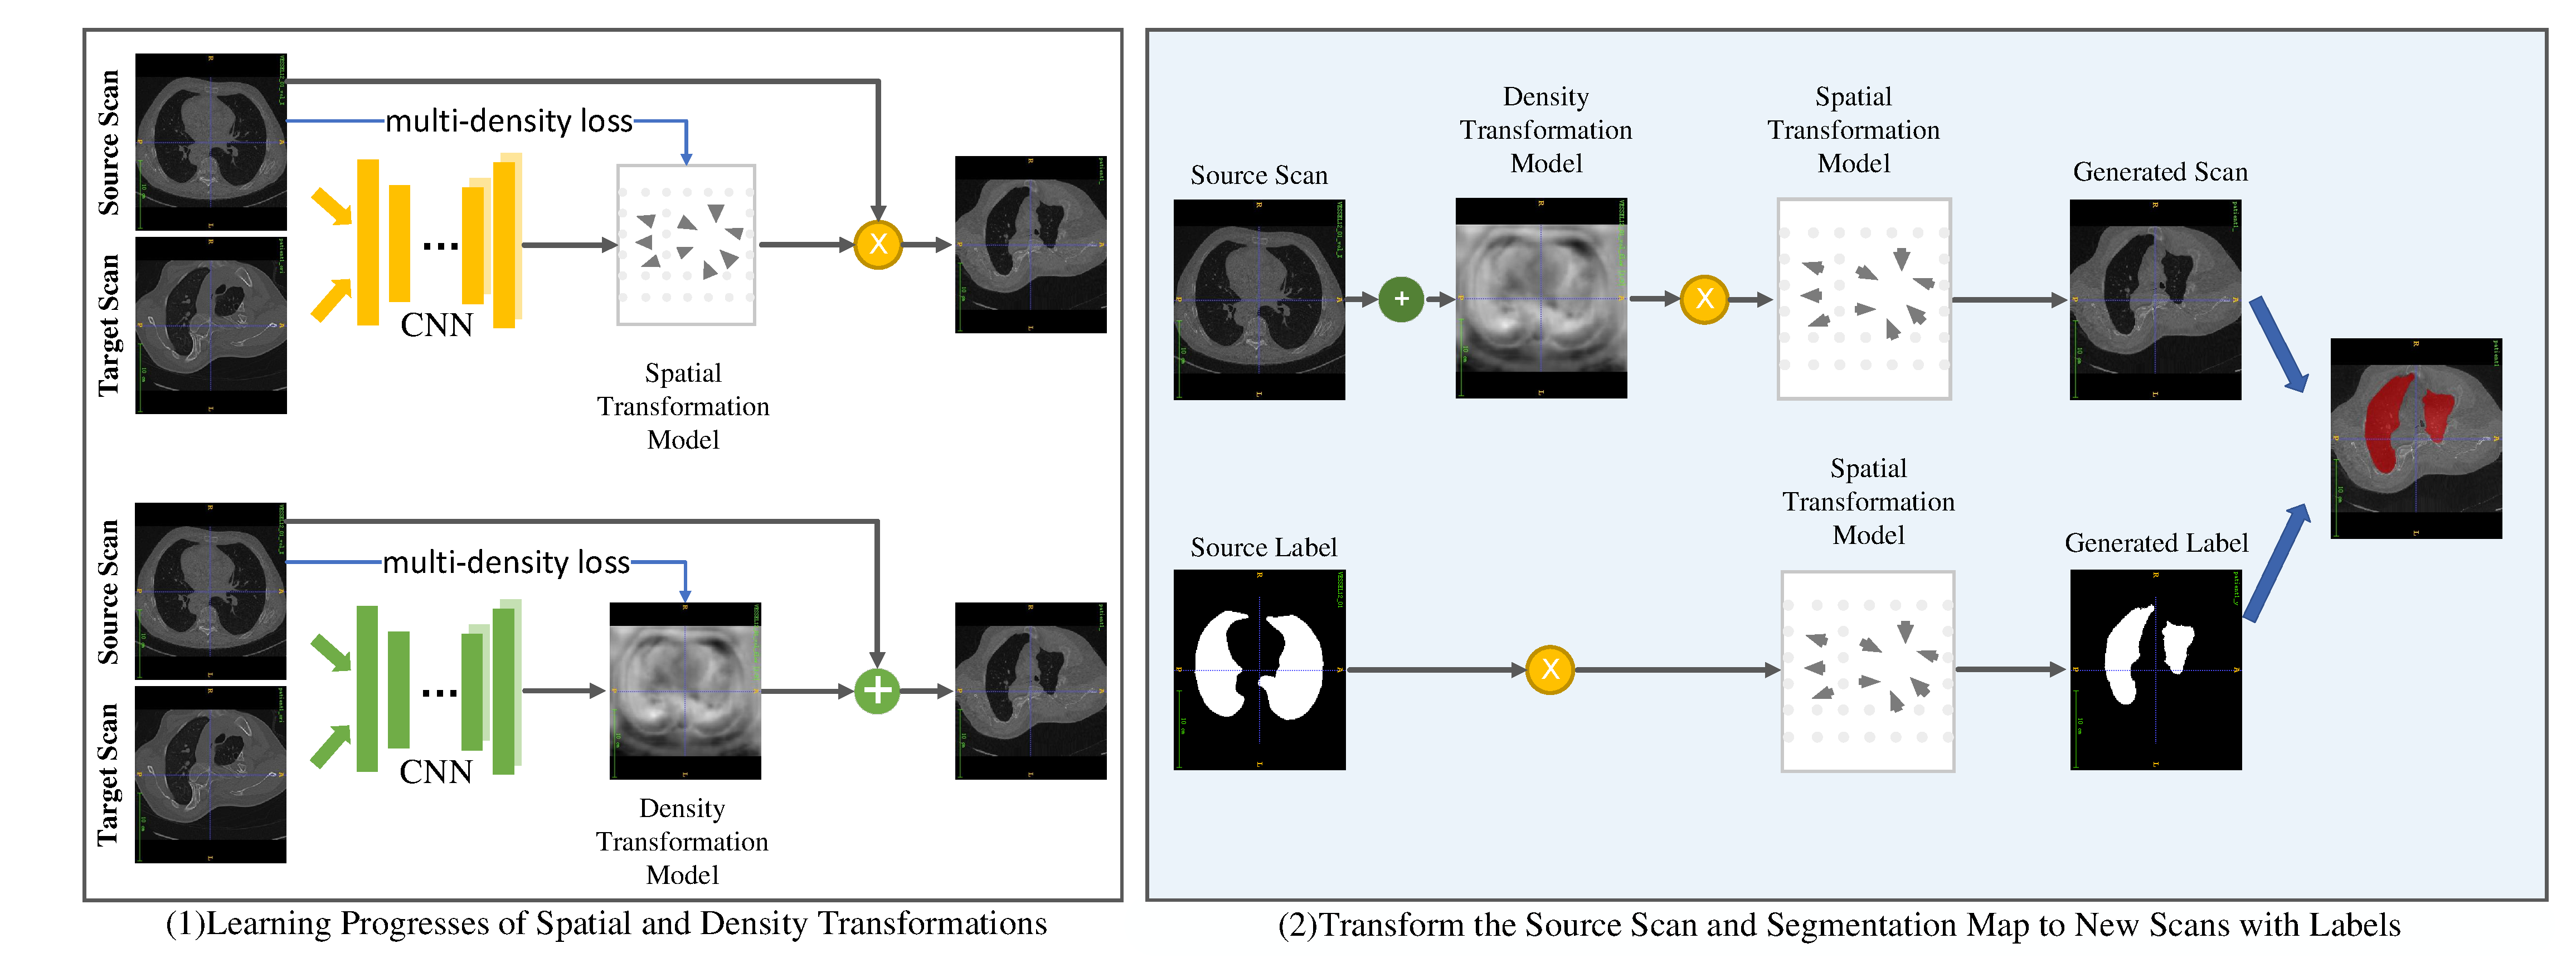
\includegraphics[width=180mm]{transarti2.pdf}}
    \vspace{-0cm}
    \caption{The overview of our framework.
    }
    \vspace{-0cm}
    \label{transarti}
    \end{figure*}


In this study, we propose a framework for one-shot lung segmentation. Our method needs only one labeled chest CT scan for VESSEL12, and generate new scans with segmentation map according to data without segmentation map.

The process of our framework is shown in Fig.~\ref{transarti}.
First, we use two U-Net models to learn the set of spatial and density transformations between the source scan and the target scans separately. Second, we apply spatial and density transformations to the source scan to synthesize new scans. Third, we apply spatial transformations to the segmentation map of the source scan to get a segmentation map for the generated new scans. Finally, we train a supervised U-Net with these generated labeled scans.


\section{Related Work}
\label{sec:related}
\subsection{Lung Segmentation}
Lung segmentation is a basic task for many studies on pulmonary diseases. Supervised methods attain state-of-the-art accuracy. Diverse works aimed to segment the lung region using different and combined techniques, that goes through region growing, border analysis, shape and probabilistic models, and recently deep learning approaches. 

Traditional methods (i.e., region growing, border analysis and so on) is mature, but have some disadvantages in medical image segmentation.
Methods like region growing \cite{adams1994seeded} relied heavily on the selection of seed points, and the segmentation speed is inefficient.
Active contour model \cite{kass1988snakes} segmentation results are greatly influenced by the initial contour setting.
Border analysis \cite{canny1987computational} performs worse when regions have no obvious boundary. 
These disadvantages limit the clinical application of these methods.

Deep learning methods, especially CNN models (Convolutional Neural Network) have been widely used to segment medical images, like U-Net \cite{ronneberger2015u}, H-DenseUNet \cite{li2018h}, 3D U-Net \cite{cciccek20163d} and so on. Jeovane H. Alves et al. Study in \cite{alves2018extracting} extract lungs from CT images using fully
convolutional networks, which achieved $96.89 \pm 3.14$ in Dice scores on VESSEL12. Ahmed Soliman et al. \cite{soliman2016accurate} achieved $99.0 \pm 0.5$ in Dice scores on VESSEL12 using adaptive appearance-guided shape modeling. Study in \cite{alves2018extracting} achieved $99.19 \pm 0.47$ in Dice sources, which is so far the state-of-art. Most deep learning methods heavily rely on labeled datasets. However, public available big-scale medical datasets are very rare, which also limits the clinical application of supervised deep learning models.

\subsection{Spatial Transformer Networks}
Spatial transformer networks \cite{jaderberg2015spatial} and its variations have been used in a variety of image analyses. Parametric spatial transform models have been used to align and classify handwritten digits \cite{hauberg2016dreaming, learned2005data, miller2000learning}. In medical image registration, a spatial deformation model is used to establish semantic correspondences between images.

Guha~Balakrishnan et al. \cite{balakrishnan2019tmi} proposed VoxelMorph, a unsupervised learning-based method, to learn spatial transformations. VoxelMorph used CNN based on U-Net to learn registration between brain MRI 3D volumes. Amy~Zhao et al. \cite{zhao2019data} proposed a method based on spatial and appearance transform. This model used two U-Net models to implement data argumentation using learned transformations for one-shot medical image segmentation. 

\section{MATERIALS AND METHODS}
\label{sec:materials}

\subsection{Datasets}
\label{dataset}
In this study, we use two datasets, which contain 110 cases.
The first dataset is VESSEL12 \cite{rudyanto2014comparing}, which was proposed for the evaluation of both semi and automatic methods for lungs’ blood vessel segmentation in CT scans. A total of 20 scans were available for testing (plus three as examples). Scans have an average of 432 slices, and each scan contains segmentation maps for lungs. This dataset is available online\footnote{https://vessel12.grand-challenge.org/}.
The second dataset is a clinical private dataset, which is collected from the Radiology Department, The First Affiliated Hospital of Army Medical University. A total of 90 scans are included. For each scan, we only keep the series under the lung window, which is one of the most common CT windows in the clinic. Since it is a private dataset, which is collected directly from the clinic, we don't have segmentation maps for each scan. 

\subsection{Methods}
\label{methods}
We propose to improve one-shot lung CT segmentation by generating new training chest CT with segmentation maps in a semi-supervised learning framework.

Following the study \cite{zhao2019data}, we use two U-Net models to learn the spatial and density transformation models. 
We first have a source scan (atlas) from VESSEL12, which has segmentation maps. Second, we use two U-Net models to learn spatial and density transformations between source scan and target scans. Third, we apply spatial and density transformations to the source scan to synthesize new scans. Third, we apply spatial transformations to the segmentation map of the source scan to get segmentation maps for the generated new scans. Finally, we train a supervised U-Net with these generated labeled scans.

We describe the differences between scans using a combination of spatial and density transformations. 
Let $T(\cdot)$ denote a transformation from one CT scan to another as a combination of a spatial transformation $t_s(\cdot)$ and a density transformation $t_d(\cdot)$. Then we have $T(\cdot)=t_s(t_d(\cdot))$. 
We model our spatial and density transformations as follows:
\begin{equation}
    t_s(x)=x\circ\mu,\qquad\qquad\mu=g\theta_s(x,y)
\end{equation}
\begin{equation}
    t_d(x)=x+\rho,\quad\rho=h\theta_d(x,y\circ\mu^{-1})
\end{equation}
We define the deformation function $\mu=id+u$, where id is the identity function, $u$ is a smooth voxel-wise displacement field. 
We use $x\circ\mu$ to denote the application of the deformation $\mu$ to $x$. In our study, $x$ is the source scan.

Then we model our appearance transform model loss as:
\begin{align*}
    L(x,y^{(i)},\mu^{(i)},\mu^{-1(i)},\rho^{(i)},c_x)=\qquad\qquad\\L_{sim}((x+\mu^{(i)})\circ\mu^{(i)}, y^{(i)})+\lambda L_{smooth}(c_x,\rho^{(i)})
\end{align*}
\begin{align*}
    L_{sim}((x+\mu^{(i)})\circ\mu^{(i)}, y^{(i)})=\quad\\\sigma_1L_{sim}((x_{bone}+\mu^{(i)})\circ\mu^{(i)}, y_{bone}^{(i)})+\\\sigma_2L_{sim}((x_{lung}+\mu^{(i)})\circ\mu^{(i)}, y_{lung}^{(i)})
\end{align*}
where $i$ indicates the $i$-th target scan. $L_{smooth}$ is a smoothness regularization function based on the segmentation map of the source scan:
\begin{equation}
    L_{smooth}=(c_x,\rho)\nabla\rho
\end{equation}
In \cite{zhao2019data}, $L_{sim}$ only calculated single loss of image similarity loss. However, their study was about brain segmentation. The density of the brain has a much smaller range than that of the lungs, so the single loss of image similarity cannot meet the requirements of lung segmentation. In our study, $L_{sim}$ is a multi-density loss, which contains loss for both CT images and bone structure. We use bone structure to improve the transformation since bones like ribs are the natural boundary for lungs. $\lambda$, $\sigma_1$ and $\sigma_2$ are parameters, which can be optimized by back-propagation algorithm.
Both density and spatial transformations are learned by separate U-Nets, as shown in Fig.~\ref{unet}.
\begin{figure*}[t]
    \centerline{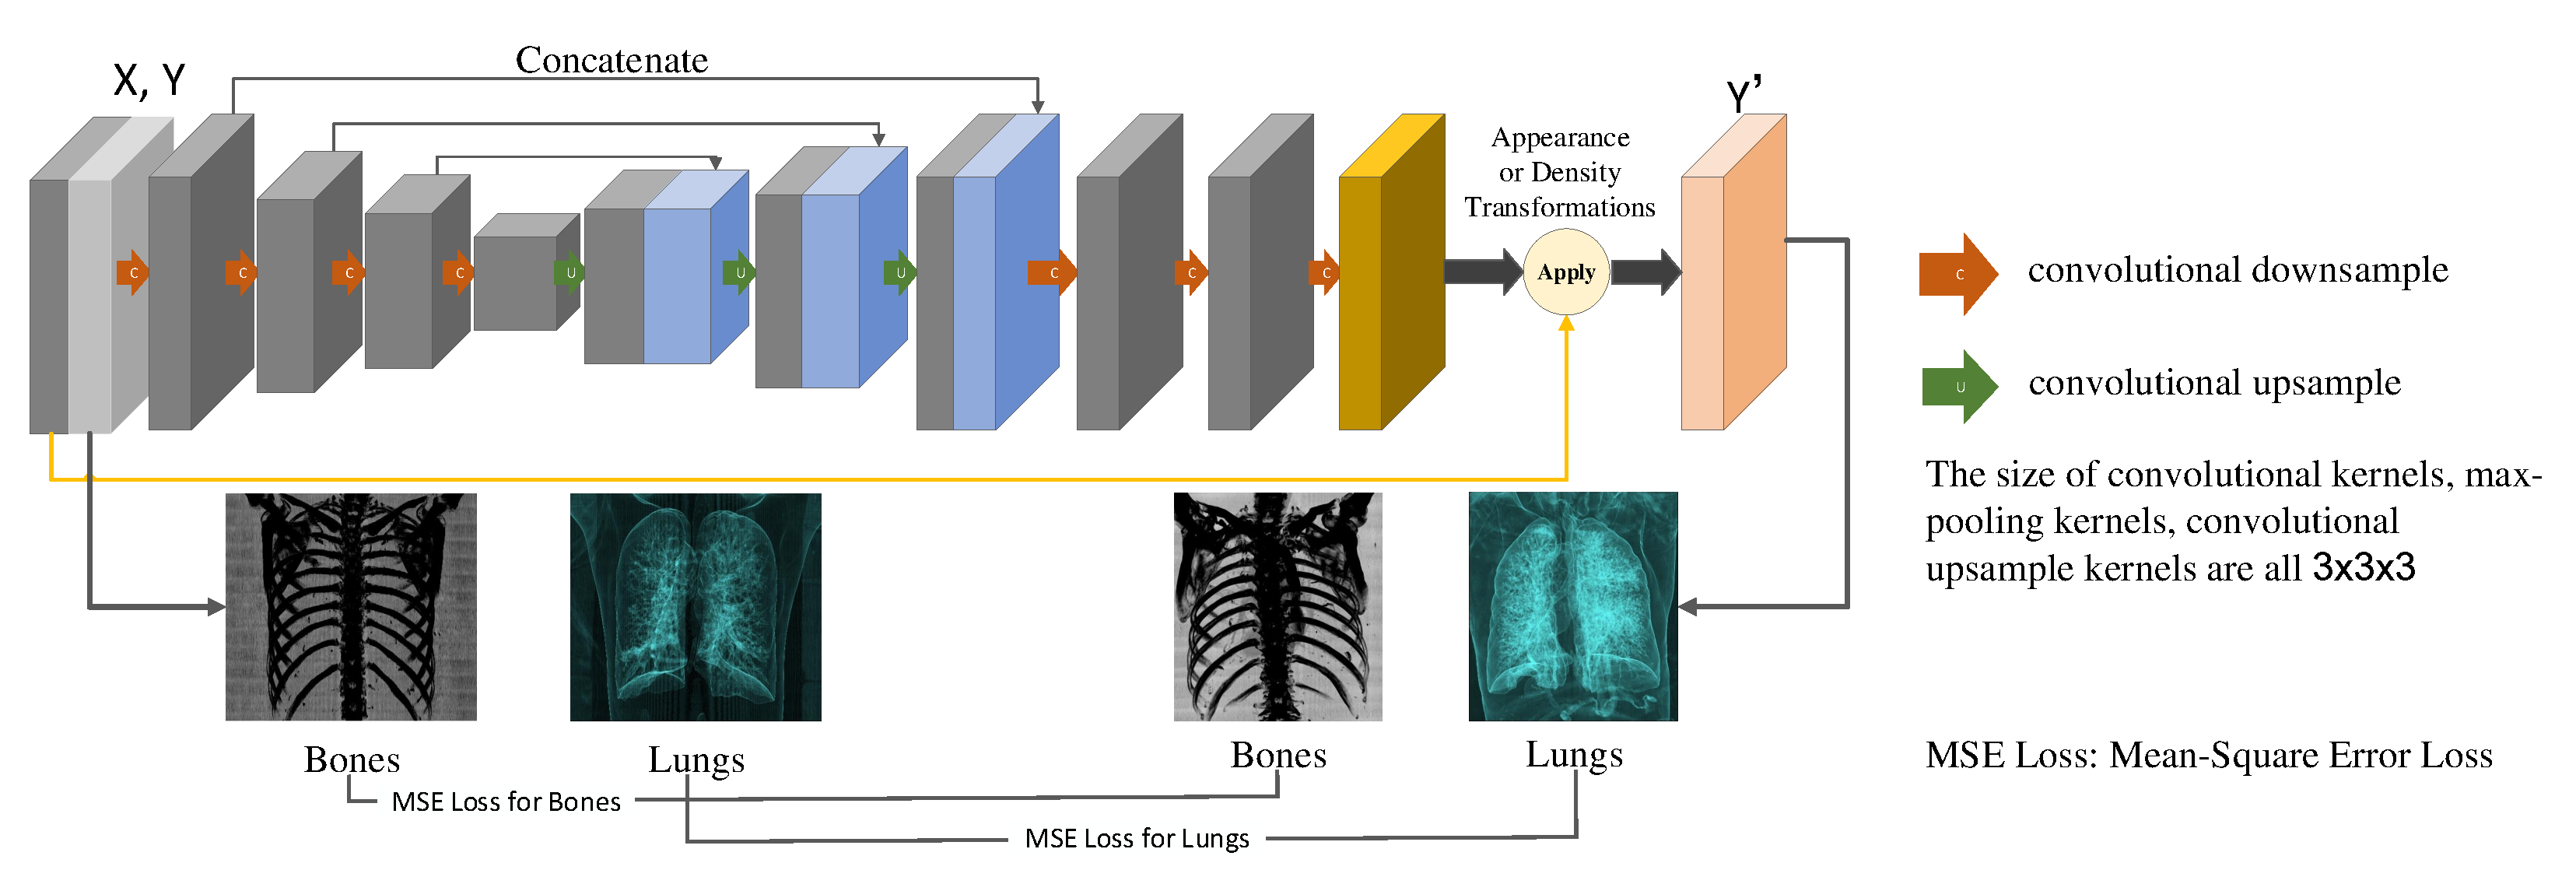
\includegraphics[width=180mm]{unet.pdf}}
    \vspace{-0cm}
    \caption{The structure of U-Net. We use this structure to learn density and spatial transformations.
    }
    \vspace{-0cm}
    \label{unet}
    \end{figure*}


\section{Experiments}
\label{sec:experiments}
In this section, we have conducted several experiments to analyze our model in details. 
In the first part of experiments, we quantitatively analyze the performance of our framework. This part of experiments are carried on with VESSEL12 since VESSEL12 provides segmentation maps for each scan.
In the second part of experiments, we verify the performance of our framework on clinical data. 
Due to the shortage of labeled data, we cannot quantitative analyze segmentation results in this part, so that we invite 2 radiologists to give subjective judgments on segmentation results.
All experiments are carried on with a GPU NVIDIA Tesla V100.

\subsection{Results on VESSEL12}
\label{subsec:vessel}
In this section, we experimentally quantitative analyze the performances our our framework on VESSEL12. Since our method requires only one segmented scan, and generate new scans which are different from VESSEL12, 20 scans are all used to verify the performances.

In these part of experiments, we conduct two experiments.
First, we pick one case and it segmentation maps as source case, and generate 20 new cases as our training set, then we train a U-Net(Ours) with these cases. We test the performance of this U-Net(Ours) on VESSEL12.
Second, we train a U-Net(One Scan) with only one segmented case (i.e., the sources case) and test the performance of this U-Net(One Scan) in the same way.

Experiments' results are listed in Table.~\ref{vesselres}. We use Dice Score (DSC) \cite{dice1945measures} to evaluate the performances of segmentation results. According to Table.~\ref{vesselres}, supervised methods have achieved verify convincing results. The state-of-art has achieved Dice Score of 99.19. The U-Net trained with only labeled scan form VESSEL12 achieves Dice Score of 91.69. The U-Net trained with generated scans achieves 96.31, 2.88 lower than the state-of-art. Considering our method requires only one segmented scan, our results are quite convincing and there is a lot of room for improvement if we have more labeled scans.

\begin{table}[htbp]    
    \caption{Comparison among Different Methods}

    \begin{center}
    \begin{tabular}{c|c|c}

    \hline
    \textbf{\textit{Methods}} & \textbf{\textit{Dataset}}& \textbf{\textit{DSC}}\\
    \hline
    Soliman et al. \cite{soliman2016accurate} & VESSEL12 & $99.00$ \\
    Alves et al. \cite{alves2018extracting} & VESSEL12 & $99.19$ \\
    \hline
    U-Net(One Scan) & VESSEL12 & $91.69$ \\
    U-Net(Ours) & VESSEL12 & $96.31$ \\
    \hline

    \end{tabular}
    \vspace{-0cm}

    \end{center}
    % \footnotesize{LW: Lung Window Image, HA: High Attenuation Image, LA: Low Attenuation Image, TC: Three-Channel Image}

    \vspace{-0cm}\    
    \label{vesselres}
    \end{table}

Moreover, we observe that some particular scans with severe diseases are difficult to segment. For example, our method only achieves Dice Score of 91.44 on VESSEL12\_17 in testing set, which lower the average score. That would be very helpful if we can get more labeled scans which have severe diseases.


\subsection{Results on Clinical Data}
\label{subsec:clinical}
In this section, we analyze the performances of our model on clinical data. We got 90 cases of chest CT, 60 cases are used to generate new data with labels, 30 cases are used to verify the segmentation results. Due to the shortage of labels of private dataset, we invite two radiologists to compare the segmentation results manually.

\begin{figure}[t]
    \centerline{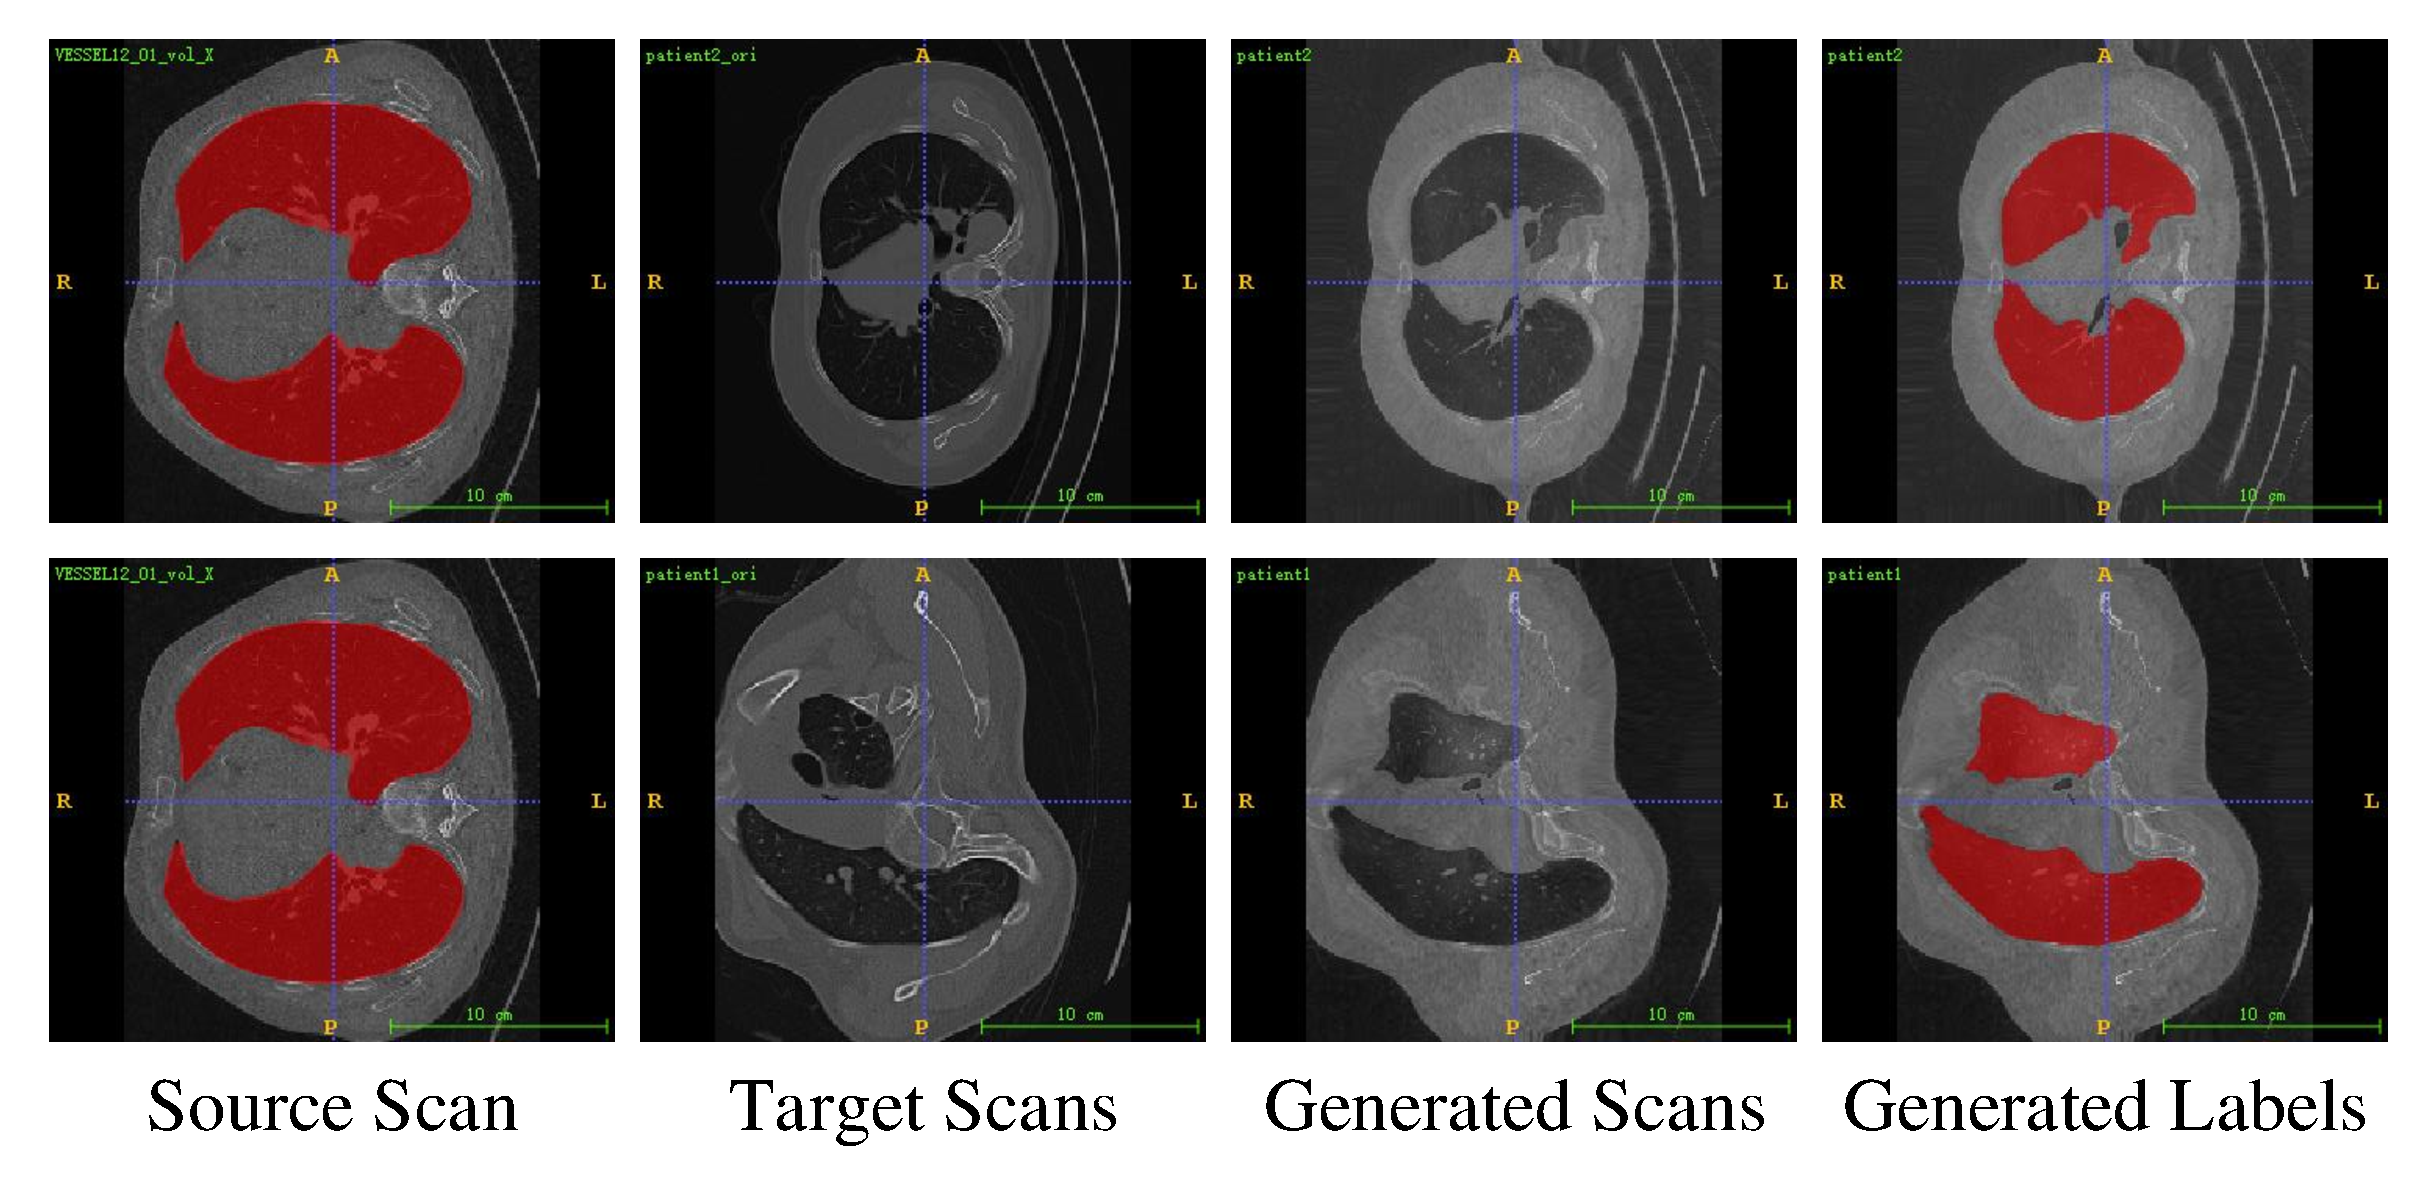
\includegraphics[width=90mm]{generatedata.pdf}}
    \vspace{-0cm}
    \caption{Comparisons between target scans, generated scans and generated labels.
    }
    \vspace{-0cm}
    \label{generatedata}
    \end{figure}

We conduct two experiments in this part.
First, we train a U-Net(VESSEL12) with all VESSEL12 data, then test this model on the testing set (30 cases).
Second, we use the source case with segmentation maps (the same as section~\ref{subsec:vessel}), and generate 60 new cases with segmentation maps. We train a U-Net(ours) and test this model one the 30 testing cases.

Due to the shortage of labeled clinical data, we first generate 60 new cases with labels. In Fig.~\ref{generatedata}, we show two generated cases with it target cases. We will release more generated cases in our website. As shown in Fig.~\ref{generatedata}, using labeled atlas form VESSEL12, we can generate new labeled scans by learning transformations. Using density and spatial transformations, atlas will be transformed in new scans, which are very similar to target scans. Then appearance transformation will be applied to labels to get new labels for generated scans. In Fig.~\ref{generatedata}, generated labels can cover lung areas in generated scans well.

After getting new scans with labels, we train a U-Net to segment lungs from clinical data. Meanwhile, we train another U-Net with VESSEL12 training data, we test these two U-Nets on 30 cases of testing data. 

Experiments demonstrate that our method can improve the performance of U-Net. Fig.~\ref{lungs} clearly shows that U-Net trained with our scans has a better performance. Our model can segment lungs better, especially these narrow areas (areas in rectangles). However, both models perform worse when lungs have severe lung diseases (the last colum).

In a word, using scans generated can improve the performances of segmenting narrow lung areas. However, since we don't have enough labeled scans which have severe diseases, both models have difficulty in segmenting lungs with diseases.


\begin{figure}[t]
    \centerline{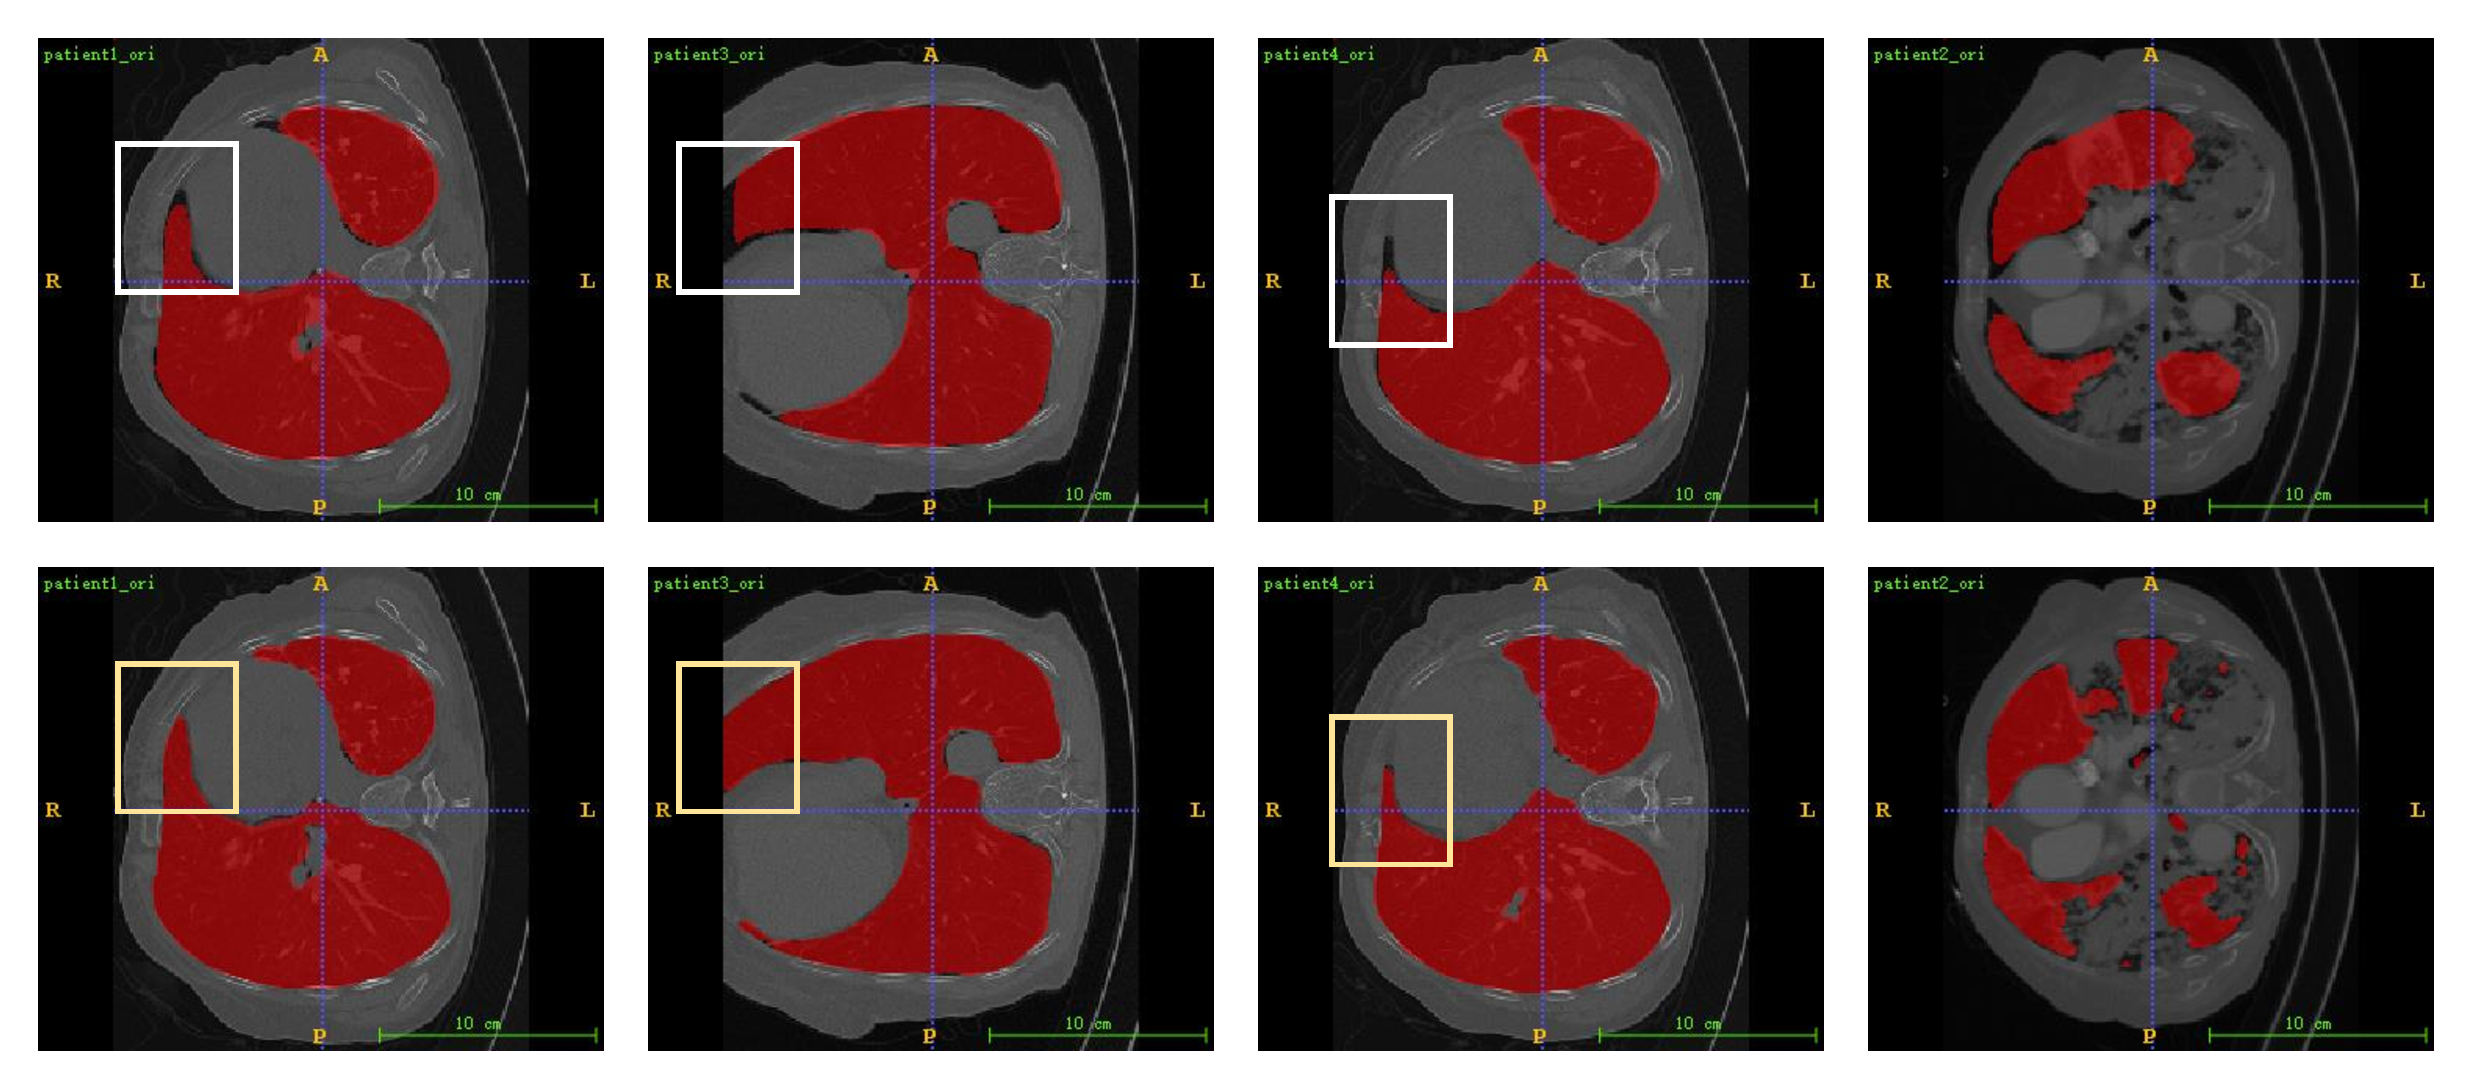
\includegraphics[width=90mm]{lungs.pdf}}
    \vspace{-0cm}
    \caption{The top row shows the segmentation results generated by a U-Net trained by VESSEL12. The bottom row shows the segmentation results generated by a U-Net trained by generated scans. 
    }
    \vspace{-0cm}
    \label{lungs}
    \end{figure}



    

% References should be produced using the bibtex program from suitable
% BiBTeX files (here: strings, refs, manuals). The IEEEbib.bst bibliography
% style file from IEEE produces unsorted bibliography list.
% -------------------------------------------------------------------------
\bibliographystyle{IEEEbib}
\bibliography{refs}

\end{document}
